\section{Puntos Críticos}

\subsection{Métricas y Utilidad}

Este script aplica un análisis de agrupamiento estadístico 
(\textit{K-Means Clustering}) 
para derivar la nueva métrica categórica ``Categoría de Peligrosidad''.
Esta m\'etrica categoriza a las zonas en: 
``Punto Crítico'', ``Precaución'' y ``Seguro / Fluido'' 
para dar un feedback visual e intuitivo al momento de mostrar los reportes.

\subsection{Lógica General}

\subsubsection*{Cargar Datos}
Se extraen las variables \texttt{indice\_riesgo} e \texttt{indice\_eficiencia}
del archivo maestro de analit\'ica espacial 
(\texttt{tramos\_analitica\_2022.csv}).
Se rellenan los valores nulos con ceros como m\'etodo de limpieza.

\subsubsection*{Clasificaci\'on con K-Means}

Se realiza un agrupamiento con \textit{K-Means}, buscando 3 clusters. Estos 
representan los 3 niveles de peligro. Luego se calcula 
\texttt{score = riesgo - eficiencia} para los centroides obtenidos, y se 
ordenan tal que un \texttt{score} mas alto, indica mayor peligro, y vice 
versa. Se asignan las etiquetas correspondientes a los clusters,
y se guardan en \texttt{puntos\_criticos\_2022.csv}.

\subsection{Reporte}

\begin{figure}[ht]
    \centerline{
        \includegraphics[page=3, scale=0.25]{graphics/reporte.pdf}
    }

    \caption{
        Reporte de los puntos cr\'iticos: \\
        (\textbf{izquierda}) Mapa de puntos, de rojo a verde
            indicando peligro (mayor a menor), y tama\~no de las burbujas 
            indicando \textit{indice\_riesgo}. 
        (\textbf{arriba-derecha}) Gr\'afica de anillo, mostrando la 
            proporci\'on de las categor\'ias asignadas. 
        (\textbf{centro-derecha}) Slicer para ver los distintos niveles de 
            peligro individualmente.
        (\textbf{abajo-derecha}) Slider para modificar los detectores mostrados 
            seg\'un el volumen de autos detectados.
    }

    \label{fig:puntos-criticos}

\end{figure}

Es interesante ver (\ref{fig:puntos-criticos}) como se encontraron tan pocos
puntos de seguridad, y 3/5 de ellos se encuentran sobre la misma avenida
`Bvar. Artigas'.
Esto demuestra grandes oportunidades de mejora, y la priorizaci\'on que se le
di\'o a Bvar. Artigas, una de las avenidas m\'as transitadas de Montevideo.

